%%%%%%%%%%%%%%%%%%%%%%%%%%%%%%%%%%%%%%%%%
% Beamer Presentation
% LaTeX Template
% Version 1.0 (10/11/12)
%
% This template has been downloaded from:
% http://www.LaTeXTemplates.com
%
% License:
% CC BY-NC-SA 3.0 (http://creativecommons.org/licenses/by-nc-sa/3.0/)
%
%%%%%%%%%%%%%%%%%%%%%%%%%%%%%%%%%%%%%%%%%

%----------------------------------------------------------------------------------------
%	PACKAGES AND THEMES
%----------------------------------------------------------------------------------------

\documentclass{beamer}

\mode<presentation> {

% The Beamer class comes with a number of default slide themes
% which change the colors and layouts of slides. Below this is a list
% of all the themes, uncomment each in turn to see what they look like.

%\usetheme{default}
%\usetheme{AnnArbor}
%\usetheme{Antibes}
%\usetheme{Bergen}
%\usetheme{Berkeley}
%\usetheme{Berlin}
%\usetheme{Boadilla}
%\usetheme{CambridgeUS}
%\usetheme{Copenhagen}
%\usetheme{Darmstadt}
%\usetheme{Dresden}
%\usetheme{Frankfurt}
%\usetheme{Goettingen}
%\usetheme{Hannover}
%\usetheme{Ilmenau}
%\usetheme{JuanLesPins}
%\usetheme{Luebeck}
\usetheme{Madrid}
%\usetheme{Malmoe}
%\usetheme{Marburg}
%\usetheme{Montpellier}
%\usetheme{PaloAlto}
%\usetheme{Pittsburgh}
%\usetheme{Rochester}
%\usetheme{Singapore}
%\usetheme{Szeged}
%\usetheme{Warsaw}

% As well as themes, the Beamer class has a number of color themes
% for any slide theme. Uncomment each of these in turn to see how it
% changes the colors of your current slide theme.

%\usecolortheme{albatross}
%\usecolortheme{beaver}
%\usecolortheme{beetle}
%\usecolortheme{crane}
%\usecolortheme{dolphin}
%\usecolortheme{dove}
%\usecolortheme{fly}
%\usecolortheme{lily}
%\usecolortheme{orchid}
%\usecolortheme{rose}
%\usecolortheme{seagull}
%\usecolortheme{seahorse}
%\usecolortheme{whale}
%\usecolortheme{wolverine}

%\setbeamertemplate{footline} % To remove the footer line in all slides uncomment this line
%\setbeamertemplate{footline}[page number] % To replace the footer line in all slides with a simple slide count uncomment this line

%\setbeamertemplate{navigation symbols}{} % To remove the navigation symbols from the bottom of all slides uncomment this line
}

\usepackage{graphicx} % Allows including images
\usepackage{booktabs} % Allows the use of \toprule, \midrule and \bottomrule in tables
\usepackage{multirow}
\usepackage{adjustbox}
\usepackage{array}
\usepackage{tikz}
\usepackage{soul}
\usetikzlibrary{shapes.geometric, arrows, positioning, fit}
\usepackage[latin1]{inputenc}
\newcommand{\xmark}{\textcolor{red}{\text{\sffamily X}}}
\newcommand{\cmark}{\textcolor{green}{\checkmark}}
\newcommand{\tr}{\text{tr}}
\newcommand{\E}{\textbf{E}}
\newcommand{\diag}{\text{diag}}
\newcommand{\argmax}{\text{argmax}}
\newcommand{\argmin}{\text{argmin}}
\newcommand{\Cov}{\text{Cov}}
\newcommand{\Var}{\text{Var}}
\newcommand{\Vol}{\text{Vol}}
\newcommand{\bx}{\boldsymbol{x}}
\newcommand{\by}{\boldsymbol{y}}
\newcommand{\bX}{\boldsymbol{X}}
\newcommand{\bY}{\boldsymbol{Y}}
\sethlcolor{gray}
\makeatletter
\newcommand\SoulColor{%
  \let\set@color\beamerorig@set@color
  \let\reset@color\beamerorig@reset@color}
\makeatother
\definecolor{color1}{RGB}{128,13,13}
\definecolor{color2}{RGB}{70,128,13}
\definecolor{color3}{RGB}{13,128,128}
\definecolor{color4}{RGB}{70,13,128}

%tikz stufff


%----------------------------------------------------------------------------------------
%	TITLE PAGE
%----------------------------------------------------------------------------------------


\title[Informal]{Causal Inference and Invariance}

\author{Charles Zheng and Qingyuan Zhao}
\institute[Stanford]
{Stanford University}
\date{\today}

\begin{document}

\begin{frame}
\titlepage
(Part 1/2)
\end{frame}

\begin{frame}
\frametitle{Understanding nature = cause and effect}
\begin{tabular}{cc}
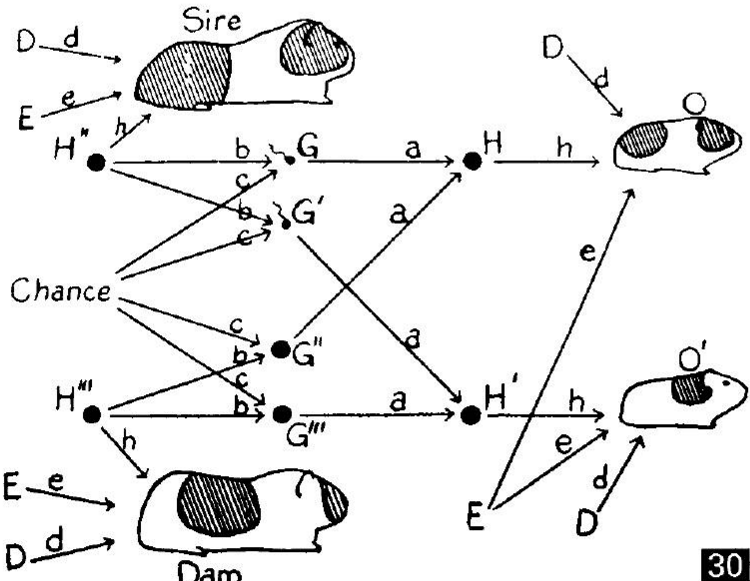
\includegraphics[scale=0.13]{../images/pearl30.png}& \\
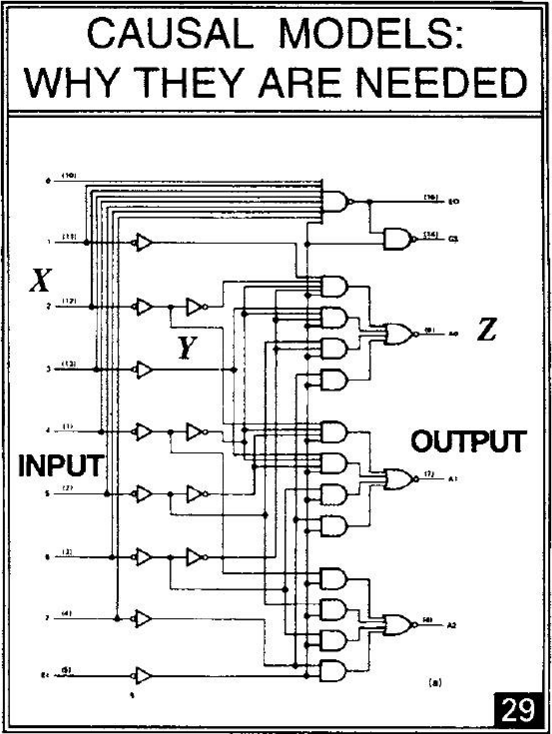
\includegraphics[scale=0.17]{../images/pearl29.png} &
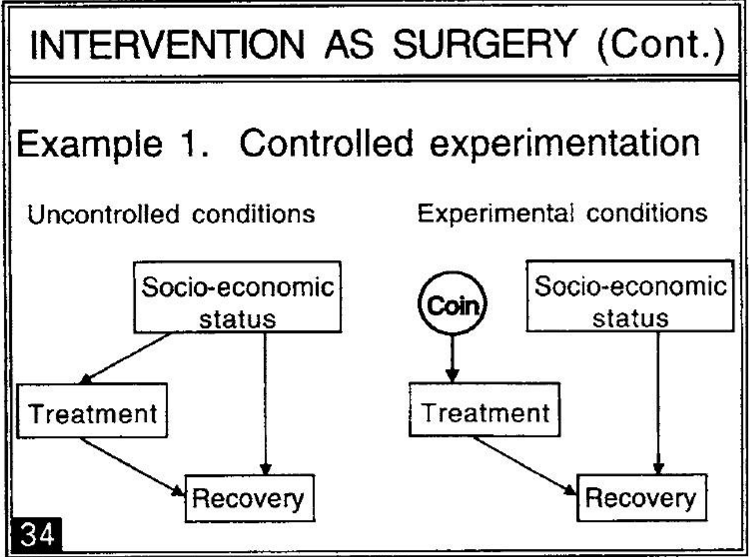
\includegraphics[scale=0.25]{../images/pearl34.png}
\end{tabular}
\end{frame}

\begin{frame}
\frametitle{A hot application: systems biology}
\begin{center}
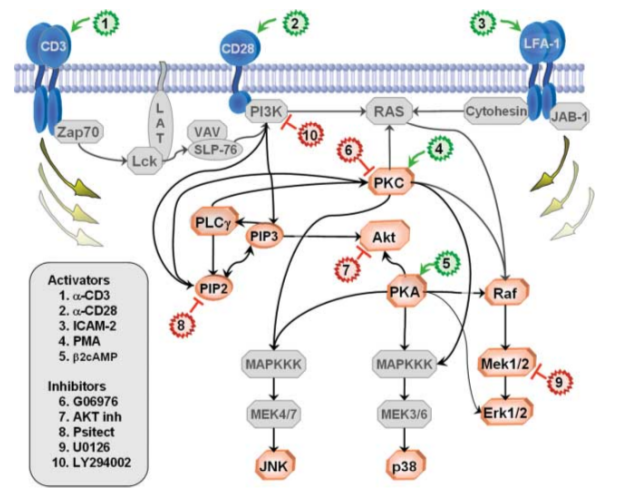
\includegraphics[scale=0.3]{../images/cyto_graph.png}
\end{center}
\begin{itemize}
\item In biology: causal relationships due to \emph{chemical interactions}.
\item Experimenters \emph{intervene} by injecting \emph{activators} and \emph{inhibitors}.
\end{itemize}
\end{frame}

\begin{frame}
\frametitle{Protein signalling data}
\begin{center}
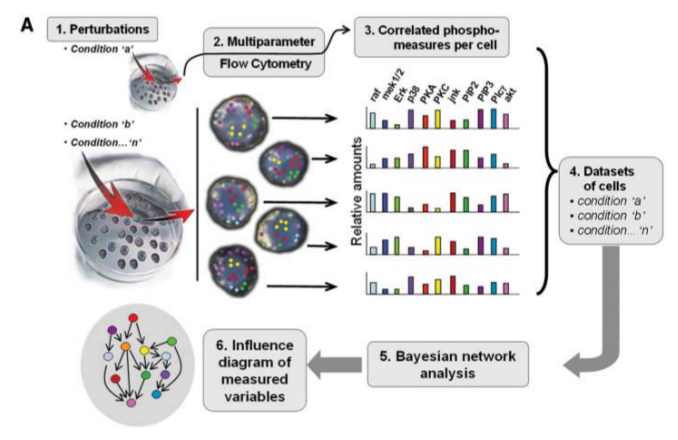
\includegraphics[scale=0.3]{../images/cytoA.png}
\end{center}
\begin{itemize}
\item Flow cytometry data from Sachs et al.\emph{Science}, 2005.
\item 1 observational data set + 9 interventions (selective activation/inhibition).
\end{itemize}
\end{frame}

\begin{frame}
\frametitle{Putative causal model}
\begin{center}
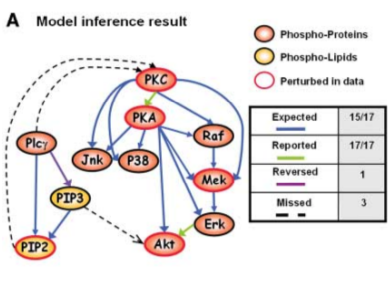
\includegraphics[scale=0.5]{../images/cyto_result_cropped.png}
\end{center}
\begin{itemize}
\item Causal inference applied to observational + interventional data.
\item Recovered most of the known interactions.
\end{itemize}
\end{frame}

\begin{frame}
\frametitle{Where does statistics fit into this?}
Not just statistics: numerous fields are interested in causal inference.
\begin{itemize}
\item \emph{Philosophy.} Starting from Aristotle and still being debated today.  What is causality?  How do we learn about cause and effect?
\item \emph{Computer science.}  Can we build an artificial intelligence which reasons like humans?  Motivation for Judea Pearl's work.
\item \emph{Social science.}  What influences an individual's life choices? (Career, political participation, etc.)  Can we discover \emph{social mechanisms}?
\end{itemize}

Statistical applications focus on:
\begin{itemize}
\item \emph{Estimating causal effects.} Can we predict a causal effect based on observational or experimental data? 
E.g. effect of a medical treatment based on clinical trial data?
Motviation for potential outcomes approach developed by Rubin, etc.
\item \emph{Bayesian networks, structure learning.} Can we model multivariate relationships using a network structure?
Networks \emph{can be} given causal interpretation, but causal inference is not the only motivation.
Motivation for graphical lasso.
\end{itemize}
\end{frame}

\begin{frame}
\frametitle{Principles of Causal Inference}

\begin{itemize}
\item These diverse applications of causal inference share a common set of useful principles.
\item The \emph{graphical approach} pioneered by Judea Pearl is the best approach for developing causal intuition.
\end{itemize}

\begin{center}
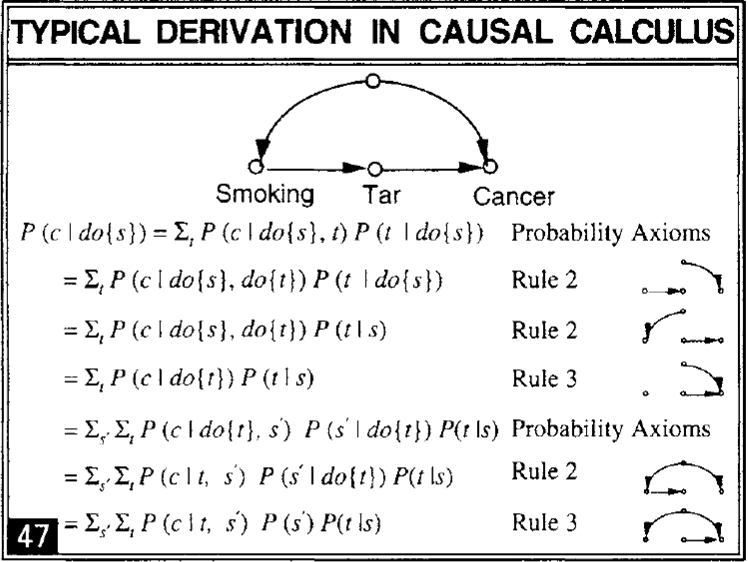
\includegraphics[scale = 0.2]{../images/pearl47.png}
\end{center}

\end{frame}

\begin{frame}
\frametitle{Graphs: nodes and vertices}

\begin{center}
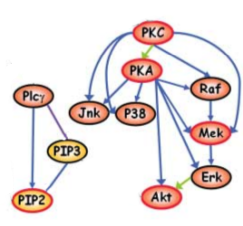
\includegraphics[scale = 0.5]{../images/cyto_result_cropped3.png}
\end{center}

\begin{itemize}
\item Each variable in the dataset is given a \emph{node}.
\item Arrows indicate which variables \emph{cause} which other variables.
\item Undirected or bidirected edges indicate that variables are associated, but neither causes the other.
\end{itemize}

\end{frame}

\begin{frame}
\frametitle{Causality and experiments}
\begin{center}
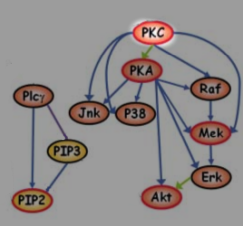
\includegraphics[scale = 0.5]{../images/fig02_01.png}
\end{center}

\begin{itemize}
\item The \emph{observational distribution} is the joint distribution under the ``natural'' state of the system.
\item One can consider \emph{intervening} on one of the variables in the system.  This changes the joint distribution of the system.
\end{itemize}

\end{frame}

\begin{frame}
\frametitle{Causality and experiments}

\begin{center}
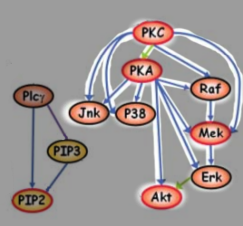
\includegraphics[scale = 0.5]{../images/fig02_02.png}
\end{center}

\begin{itemize}
\item However, not every variable will be affected by the intervention!
\item By following the arrows, we determine the set of variables which are affected by the intervention.
\end{itemize}

\end{frame}



\begin{frame}
\frametitle{Look!  A diagram!}
Don't put this in the final presentation.

\begin{center}
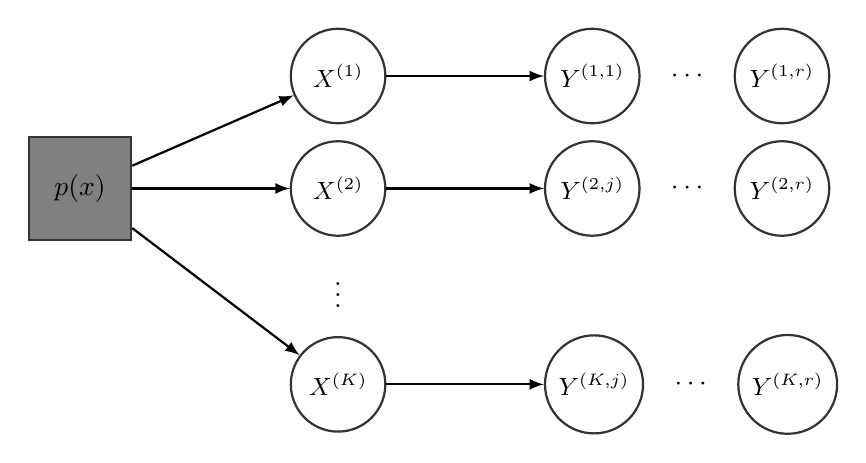
\begin{tikzpicture}[node distance = 2mm and 20mm]
\tikzstyle{main} = [circle, minimum size = 12mm, thick, draw = black!80]
\tikzstyle{main0} = [circle, minimum size = 2mm, thick, draw = white!100]
\tikzstyle{param} = [rectangle, minimum size = 13mm, thick, draw = black!80]
\tikzstyle{connect} = [-latex, thick]
\tikzstyle{box} = [rectangle, draw = black!100]
  \node[param, fill = black!50] (px) {$p(\bx)$};
  \node[main, right=of px] (x2) {\small{$\bX^{(2)}$}};
  \node[main, above=of x2] (x1) {\small{$\bX^{(1)}$}};
  \node[main0, below=of x2] (xdots) {$\vdots$};
  \node[main, below=of xdots] (x3) {\small{$\bX^{(K)}$}};
  \node[main, right=of x1] (y11) {\small{$\bY^{(1,1)}$}};
  \node[main, right=of x2] (y21) {\small{$\bY^{(2,j)}$}};
  \node[main, right=of x3] (y31) {\small{$\bY^{(K,j)}$}};
\begin{scope}[node distance = 3mm and 2mm]
  \node[main0, right=of y11] (y12) {$\cdots$};
  \node[main0, right=of y21] (y22) {$\cdots$};
  \node[main0, right=of y31] (y32) {$\cdots$};
  \node[main, right=of y12] (y13) {\small{$\bY^{(1,r)}$}};
  \node[main, right=of y22] (y23) {\small{$\bY^{(2,r)}$}};
  \node[main, right=of y32] (y33) {\small{$\bY^{(K,r)}$}};
\end{scope}
\path (px) edge [connect] (x1) (px) edge [connect] (x2) (px) edge [connect] (x3)
      (x1) edge [connect] (y11) (x2) edge [connect] (y21) (x3) edge [connect] (y31);
\end{tikzpicture}
\end{center}

\begin{center}


Legend: $K = \{$
\sethlcolor{color1}
\textbf{\textcolor{white}{\SoulColor\hl{ 2 }}}, 
\sethlcolor{color2}
\textbf{\textcolor{white}{\SoulColor\hl{ 9 }}},
\sethlcolor{color3}
\textbf{\textcolor{white}{\SoulColor\hl{ 99 }}},
\sethlcolor{color4}
\textbf{\textcolor{white}{\SoulColor\hl{ 999 }}}$\ \}$
\end{center}


\end{frame}




\end{document}






